%%%%%%%% ICML 2018 EXAMPLE LATEX SUBMISSION FILE %%%%%%%%%%%%%%%%%

\documentclass{article}

% Recommended, but optional, packages for figures and better typesetting:
\usepackage{microtype}
\usepackage{graphicx}
\usepackage{caption}
\usepackage{subcaption}
\usepackage{booktabs} % for professional tables

% hyperref makes hyperlinks in the resulting PDF.
% If your build breaks (sometimes temporarily if a hyperlink spans a page)
% please comment out the following usepackage line and replace
% \usepackage{icml2018} with \usepackage[nohyperref]{icml2018} above.
\usepackage{hyperref}

% Attempt to make hyperref and algorithmic work together better:
\newcommand{\theHalgorithm}{\arabic{algorithm}}

% Use the following line for the initial blind version submitted for review:
\usepackage{icml2018}
\usepackage{natbib}
\usepackage{amsmath}
\usepackage{amsthm}
\usepackage{amsfonts}
\usepackage{bbm}
\usepackage{bm}
\usepackage{amssymb}
\usepackage{enumitem}
\newtheorem{theorem}{Theorem}
\newtheorem{proposition}[theorem]{Proposition}
\newtheorem{definition}{Definition}
\makeatletter
\renewenvironment{proof}[1][\proofname]{\par
  \vspace{-\topsep}% remove the space after the theorem
  \pushQED{\qed}%
  \normalfont
  \topsep0pt \partopsep0pt % no space before
  \trivlist
  \item[\hskip\labelsep
        \itshape
    #1\@addpunct{.}]\ignorespaces
}{%
  \popQED\endtrivlist\@endpefalse
  \addvspace{0pt plus 0pt} % some space after
}
\makeatother

% Supplementary File
\usepackage{xr-hyper}
\externaldocument[Su-]{Supplementary}

% If accepted, instead use the following line for the camera-ready submission:
%\usepackage[accepted]{icml2018}

% The \icmltitle you define below is probably too long as a header.
% Therefore, a short form for the running title is supplied here:
\icmltitlerunning{Incentivizing High Quality Crowdsourcing Information using Bayesian Inference and Reinforcement Learning}

\begin{document}

\twocolumn[
\icmltitle{Incentivizing High Quality Crowdsourcing Information using\\Bayesian Inference and Reinforcement Learning}

% It is OKAY to include author information, even for blind
% submissions: the style file will automatically remove it for you
% unless you've provided the [accepted] option to the icml2018
% package.

% List of affiliations: The first argument should be a (short)
% identifier you will use later to specify author affiliations
% Academic affiliations should list Department, University, City, Region, Country
% Industry affiliations should list Company, City, Region, Country

% You can specify symbols, otherwise they are numbered in order.
% Ideally, you should not use this facility. Affiliations will be numbered
% in order of appearance and this is the preferred way.
\icmlsetsymbol{equal}{*}

\begin{icmlauthorlist}
\icmlauthor{Zehong Hu}{NTU}
\icmlauthor{Yang Liu}{Harvard}
\icmlauthor{Yitao Liang}{UCLA}
\icmlauthor{Jie Zhang}{NTU}
\end{icmlauthorlist}

%\icmlaffiliation{NTU}{Rolls-Royce Cooperate Lab@NTU, School of Computer Science and Engineering, Nanyang Technological University, Singapore}
%\icmlaffiliation{goo}{Googol ShallowMind, New London, Michigan, USA}
%\icmlaffiliation{ed}{School of Computation, University of Edenborrow, Edenborrow, United Kingdom}

%\icmlcorrespondingauthor{Cieua Vvvvv}{c.vvvvv@googol.com}
%\icmlcorrespondingauthor{Eee Pppp}{ep@eden.co.uk}

% You may provide any keywords that you
% find helpful for describing your paper; these are used to populate
% the "keywords" metadata in the PDF but will not be shown in the document
\icmlkeywords{Machine Learning, ICML}

\vskip 0.3in
]

% this must go after the closing bracket ] following \twocolumn[ ...

% This command actually creates the footnote in the first column
% listing the affiliations and the copyright notice.
% The command takes one argument, which is text to display at the start of the footnote.
% The \icmlEqualContribution command is standard text for equal contribution.
% Remove it (just {}) if you do not need this facility.

%\printAffiliationsAndNotice{}  % leave blank if no need to mention equal contribution
%\printAffiliationsAndNotice{} % otherwise use the standard text.

\begin{abstract}
This document provides a basic paper template and submission guidelines.
Abstracts must be a single paragraph, ideally between 4--6 sentences long.
Gross violations will trigger corrections at the camera-ready phase.
\end{abstract}

\section{Introduction}
\subsection{Motivation}
Peer prediction mechanisms have two fatal drawbacks:
\begin{itemize}
\item Existing peer prediction mechanisms only care about incentive compatibility (IC) which only poses requirements to the expected incentives to workers. They achieve IC via comparing the reports between the targeted and selected reference agents. In this way, they only use a tiny part of the information behind all collected labels. Besides, they never analyze the stochastic property of incentives and the variation of incentives among different types of agents.
\item Existing peer prediction mechanisms simplify workers' responses to the incentive mechanism by assuming that workers are all fully rational and only follow the utility-maximizing strategy. However, there is strong evidence showing that human workers are not always fully rational, and they may deviate from equilibrium strategies. Thus, these peer prediction mechanisms which is fancy in theory may yet fail in practice.
\end{itemize}

\subsection{Contribution}
We have two core contributions in this paper:
\begin{itemize}
\item We propose a novel one-shot peer prediction mechanism based on Bayesian inference. Since existing Bayesian inference algorithms (e.g. EM estimator and variational inference) for crowdsourcing are biased in principle, we derive the explicit posterior distribution of the true labels and employ Gibbs sampling for inference. The most challenging problem of our mechanism is to prove the incentive compatibility of our mechanism which has never been explored in the literature. Besides, we also empirically show the advantages of our mechanism on the stability and fairness of incentives over existing ones.
\item We design the first reinforcement peer prediction framework which sequentially interacts with workers. It dynamically adjusts the scaling level of our peer prediction mechanism to maximize the utility of the data requester. To avoid assuming a decision-making model for workers, we use the data-driven Gaussian process to represent the scaling level adjustment policy, and online updates our policy according to workers' responses. We theoretically prove the incentive compatibility of our framework and empirically show its advantages on improving the utility if the data requester over one-shot mechanisms.
\end{itemize}

\section{Related Work}

\newpage
\section{Problem Formulation}
\label{PF}
Suppose there is one data requester who assigns $M$ tasks with answer space $\left\{1,2\right\}$ to $N \geq 3$ candidate workers at each time step $t=1,2\ldots$.
We denote the tasks and workers by $\mathcal{T}^{t}=\{1,2,\ldots,M\}$ and $\mathcal{C}=\{1,2,\ldots,N\}$, respectively.
Meanwhile, we use $L^{t}_{i}(j)$ to denote the label generated by worker $i\in \mathcal{C}$ for task $j\in\mathcal{T}^{t}$.
If $L^{t}_{i}(j)=0$, we mean that task $j$ is not assigned to worker $i$ at step $t$.

The generated label $L^{t}_{i}(j)$ depends both on the ground-truth label $L^{t}(j)$ and worker $i$'s effort level $e^{t}_i$ and reporting strategy $r^{t}_i$.
Any worker $i$ can potentially have two effort levels, High ($e^{t}_i=1$) and Low ($e^{t}_i=0$).
Also, he/she can decide either to truthfully report his observation $r^{t}_i = 1$ or to revert the answer $r^{t}_i = 0$.
Workers may act differently for different tasks. 
We thus define $e^{t}_i\in[0,1]$ and $r^{t}_i\in[0,1]$ as worker $i$'s probability of exerting high efforts and being truthful, respectively.
In this case, worker $i$'s probability of being correct (PoBC) can be computed as
\begin{equation}
\begin{split}
&p^{t}_i=r^{t}_i e^{t}_i p_{i, H}+r^{t}_i (1-e^{t}_i) p_{i, L}+\\
&(1-r^{t}_i) e^{t}_i (1-p_{i, H})+(1-r^{t}_i) (1-e^{t}_i) (1-p_{i, L})
\end{split}
\end{equation}
where $p_{i, H}$ and $p_{i, L}$ denote worker $i$'s probability of observing the correct label when exerting high and low efforts, respectively.
Following \cite{dasgupta2013crowdsourced,liu2017sequential}, we assume that the tasks are homogeneous and the workers share the same set of $p_{i, H}, p_{i, L}$, denoting by $p_H, p_L$, and $p_{H}>p_{L}= 0.5$.
Here, $p^t_i=0.5$ means that worker $i$ randomly selects a label to report.

The data requester needs to pay each worker some money as the incentive for providing labels.
We denote the payment for worker $i$ at step $t$ as $P^{t}_{i}$.
At the beginning of each time step, the data requester promises the workers a certain rule of payment determination which acts the contract between two sides and cannot be changed until the next time step.
The workers are self-interested and may change their reporting strategies ($e^t_i$ and $r^t_i$) according to the payment rule.
Workers' different reporting strategies will lead to the different values of workers' PoBCs and finally different levels of label quality.
After collecting the labels from the workers, the data requester will infer the true labels by using a certain inference algorithm, and \cite{zheng2017truth} provide a good survey of existing inference algorithms.
Denote the the inferred true label of task $j$ by $\tilde{L}^{t}(j)$.
Then, the label accuracy $A^t$ and the utility $u^t$ of the data requester satisfy
\begin{equation}
\label{utility}
\begin{split}
A^t&=\frac{1}{M}{\sum}_{j=1}^{M}1\left[\tilde{L}^{t}(j)=L^{t}(j)\right]\\
u^t &= F(A^t) - \eta {\sum}_{i=1}^{N}P^t_i
\end{split}
\end{equation}
where $F(\cdot)$ is a non-decreasing monotonic function mapping accuracy to utility and $\eta$ is a
tunable parameter balancing label quality and costs. Intuitively, the $F(\cdot)$ function needs to be non-deceasing as higher accuracy is preferred.

The number of tasks in crowdsourcing is often very large, and the interaction between tasks and workers may last for hundreds of time steps.
Thus, we introduce the cumulative utility $U(t)$ of the data requester from the current step $t$ as
\begin{equation}
U(t)={\sum}_{k=t}^{\infty}\rho^{k-t}u^t
\end{equation}
where $0\leq \rho< 1$ is the discount factor which determines the importance of future utilities.
The objective of our study is to maximize $U(t)$ by optimally designing the payment rule and the ex-post adjustment algorithm of the payment rule, which we call as the incentive mechanism.

%Note our framework is robust to any such $F(\cdot)$ function. For instance, we set it as $F(A_t)=A^{10}_t$ in our experiments.



%At the beginning of each time step, the data requester will promise the workers a certain rule of payment determination.
%The workers are self-interested and may change their reporting strategies ($e^t_i$ and $r^t_i$) according to the payment rule.
%We can only adjust the payment rule after the payment is finished.
%Our objective is to maximize $U(t)$ by optimally deciding the payment for workers.



%Thus, our objective is to maximize $U(t)$ by optimally adjusting the payment $P_i^t$.
%Different from the common closed-loop control systems, crowdsourcing markets require the payment rule to be announced beforehand and cannot be changed before the next time step.
%Besides, we need to interact with $N$ self-interested workers at the same time, which also makes the .
%
%This difference motives us to firstly design a utility-maximizing payment rule by assuming workers only to take the payment-maximizing strategy. 
%Then, we develop an algorithm to adjust the payment rule after the payment is finished so that the long-term utility will also be maximized.
%In this paper, we call the payment rule and the ex-post adjustment algorithm as the incentive mechanism.


\begin{figure}[t]
 	\centering
	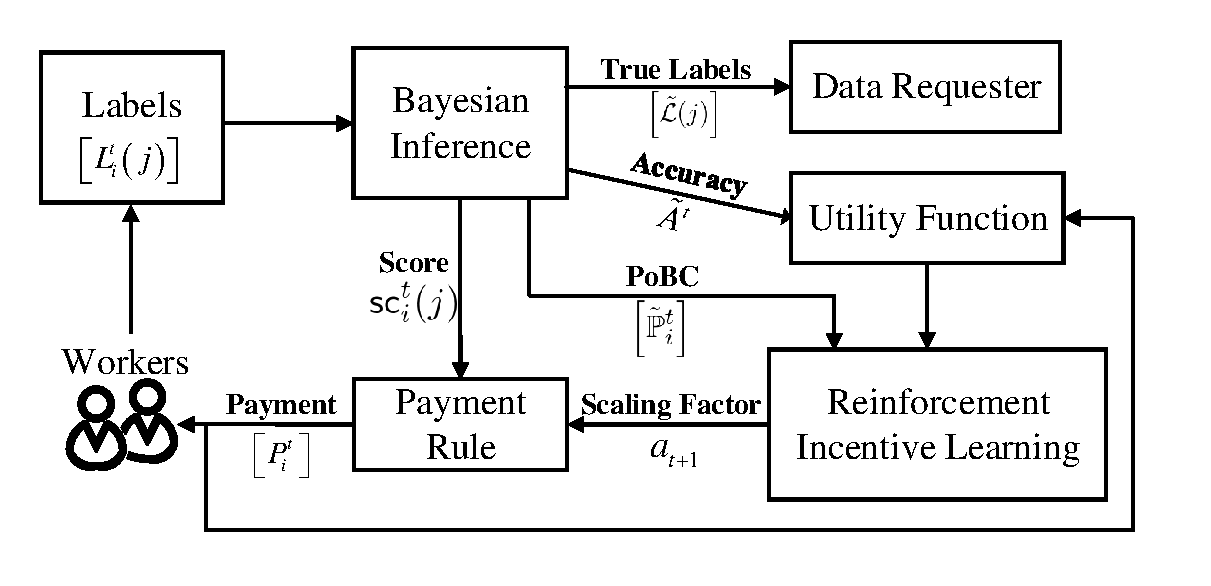
\includegraphics[width=0.48\textwidth]{image/Architecture}
	\vspace*{-8mm}
    \caption{\label{Archi} Architecture of our incentive mechanism}
\end{figure}
\section{Incentive Mechanism for Crowdsourcing}
We present the architecture of our incentive mechanism in Figure~\ref{Archi}, where the estimate of a variable is denoted by adding an over-tilde.
In our incentive mechanism, the Bayesian inference algorithm is responsible for estimating the true labels, workers' PoBCs and the label accuracy based on the collected labels at each time step.
The payment rule is designed to ensure that reporting truthfully ($r^{t}_i = 0$) and exerting high efforts ($e^{t}_i=1$) is the payment-maximizing strategy for all workers at any time step.
By doing so, we wish to induce workers to generate high-quality labels and thus improve the label accuracy.
The reinforcement adjustment algorithm adjusts the payment rule based on the historical data of payments, workers' PoBCs and label accuracy.
In this way, we can optimally balance the utility got from the labels and lost in the payments, which corresponds to $F(A^t)$ and $\sum_{i}P_i^t$ in Equation~\ref{utility}, respectively.
Besides, our incentive mechanism can ensure that always reporting truthfully ($r^{t}_i \equiv 0$) and exerting high efforts ($e^{t}_i \equiv 1$) is the payment-maximizing strategy for workers in the long term.
This property prevents the clever manipulation which earns higher long-term benefits by sacrificing short-term ones.

Nevertheless, there are three challenges to achieve our design. Firstly, our empirical studies reveal that popular inference algorithms may be heavily biased on estimating the label accuracy when the quality of labels is very low. For example, when there are $10$ workers and $q_i^t=0.55$, the estimated label accuracy of the EM estimator~\cite{dawid1979maximum,raykar2010learning} stays at around $0.9$ while the real accuracy is only around $0.5$.
This heavy bias will cause the utility to be miscalculated and thus mislead our reinforcement adjustment.
To reduce the inference bias, we develop our Bayesian inference algorithm by introducing the soft Dirichlet priors for both the true labels and workers' PoBCs.
In this case, the posterior distribution cannot be expressed as any known distributions, which motivates us to derive the explicit posterior distribution at first and then employ Gibbs sampling to conduct inference.
{\color{red}Secondly, the reinforcement adjustment expects the utility to be accurately calculated so that the direction of adjustment is clear.
However, both the label accuracy and workers' PoBCs in our incentive mechanism are corrupted by noise.
Considering that these estimates are calculated as an average over $M$ tasks, the central limit theorem ensures that the inference noise approaches the Gaussian distribution.
Therefore, to overcome the inference noise, we develop our reinforcement adjustment algorithm based on the Gaussian process.}
Lastly, the biggest challenge of our study is to prove that our incentive mechanism can ensure that reporting truthfully and exerting high efforts is the payment-maximizing strategy for workers in not only each time step and but also the long term.
For clarity, we put the theoretical analysis in the next section.
In this section, we focus on the first two challenges.


%Figure~\ref{Archi} shows the architecture of our incentive framework.
%Different from industrial feedback control systems, crowdsourcing markets require the data requester to announce the incentive mechanism to workers before allocating tasks to workers, which is actually a contract between two sides.
%So, we design our framework as two levels.
%The inner level is the Bayesian incentive mechanism which is always open to workers.
%Its objective is to ensure that reporting truthfully and exerting high efforts are the optimal strategy for all workers at any time step $t$.
%By doing so, we expect that all workers are fully rational and can follow this optimal strategy.
%However, in practice, human workers may not always fully rational and can even learn from the interactions with our mechanism.
%Thus, we develop the outer level, the reinforcement incentive mechanism, which adjusts the scaling level $a^t$ of our Bayesian mechanism to maximize the long-term utility of the data requester.
%Meanwhile, our reinforcement incentive mechanism must also ensure that reporting truthfully and exerting high efforts are the optimal strategy for workers in the long term.
%In this way, we can prevent the manipulation of any single worker.




\subsection{Payment Rule}
Suppose, at time step $t$, worker $i$ finishes $M^{t}_{i}$ tasks.
Then, the payment for worker $i$ should be
\begin{equation}
P^t_i=M_i^t\cdot (a^t r^{t}_i+b)\;\; , \;\; \phi^{t}_i = \tilde{p}^{t}_i - 0.5
\end{equation}
where we call $\phi^{t}_i$ as worker $i$'s score and $\tilde{p}^{t}_i$ will be calculated by our Bayesian inference algorithm.
$a^t$ is the scaling factor. 
It is determined by our reinforcement adjustment algorithm at the beginning of step $t$.
We denote all the available values of $a^t$ as set $\mathcal{A}$.
Besides, $b\geq 0$ is the fixed base payment.


\subsection{Bayesian Inference}
%An accurate inference algorithm, which is responsible for estimating $L^{t}(j)$, $p^t_i$ and $A^t$, is the foundation of our framework. There have been many inference algorithms developed in the literature~\cite{zheng2017truth}. Among them, two popular ones are the EM estimator~\cite{dawid1979maximum} and the variational inference estimator~\cite{liu2012variational}.
%However, our empirical studies in Figure~\ref{BIM1} reveal that these iterative estimators, which may converge to the local optimum, will be heavily biased when the quality of labels is very low.
%Thus, we employ the similar Dirichlet priors as the variation inference estimator but explicitly derive the posterior distribution of true labels rather than relying on the evidence lower bound~\cite{blei2017variational}.
%Then, we use Gibbs sampling to efficiently sample the posterior distribution to calculate the estimates of $L^{t}(j)$, $p^t_i$ and $A^t$.

%since the EM estimator may converge to the local optimum.
%On the other hand, sampling-based Bayesian inference algorithms, for example Gibbs sampling, are computationally very expensive, even though they use the explicit posterior distribution and can avoid the inference bias.
%Especially, workers' scores are continuous variables, which will significantly slow down the convergence speed.
%Therefore, to the best of my knowledge, sampling-based Bayesian inference is never used for crowdsourcing where the number of workers and tasks is usually very large.
%In this section, to reduce the inference bias and meanwhile avoid overly large computation costs, we firstly assume Dirichlet priors for those continuous variables in our system and derive a joint posterior distribution which only contains the discrete variables.
%Then, we use Gibbs sampling to sample the obtained posterior distribution and estimate workers' scores based on those samples.

%\footnote{In practice, $M^{t}_{i}$ is often smaller than $M$, and we can introduce $L^{t}_i(j)=0$ to denote that task $j$ is not assigned to worker $i$. The incentive mechanisms developed in this paper can work well in the case where the matrix $[L^{t}_i(j)]$ is sparse. However, to simplify the theoretical analysis, we assume $M^{t}_{i}\equiv M$ in this paper and put the theoretical analysis on the sparse case as our future work.}

Now, we present the details of our inference algorithm. For the simplicity of notations, we omit the superscript $t$ in this subsection. The joint distribution of the collected labels $\mathcal{L}=[L_i(j)]$ and the true labels $\bm{L}=[L(j)]$ satisfies
\begin{equation}
\label{JointDist}
\begin{split}
    &P(\mathcal{L},\bm{L}| \bm{p}, \bm{\tau})=\\ &\qquad {\prod}_{j=1}^{M}{\prod}_{k=1}^{K}\left\{\tau_{k}\prod_{i=1}^{N}p_i^{\delta_{ijk}}(1-p_i)^{\delta_{ij(3-k)}} \right\}^{\xi_{jk}}
\end{split}
\end{equation}
where $\bm{p}=[p_i]_N$ and $\bm{\tau}=[\tau_1,\tau_2]$. $\tau_1$ and $\tau_2$ denote the distribution of answer $1$ and $2$ among all tasks, respectively.
Besides,  $\delta_{ijk}=\mathbbm{1}(L_i(j)=k)$ and $\xi_{jk}= \mathbbm{1}(L(j)=k)$.
Here, we assume Dirichlet priors $\textrm{Dir}(\cdot)$ for $p_i$ and $\bm{\tau}$ as
\begin{equation}
[p_{i}, 1-p_i]\sim \textrm{Dir}(\alpha_{1},\alpha_{2})\;,\; \bm{\tau}\sim \textrm{Dir}(\beta_{1},\beta_{2}).
\end{equation}
Then, the joint distribution of $\mathcal{L}$, $\bm{L}$, $\bm{p}$ and $\bm{\tau}$ satisfies
\begin{equation}
\label{JointDist2}
\begin{split}
&P(\mathcal{L},\bm{L},\bm{p}, \bm{\tau}|\bm{\alpha}, \bm{\beta})=P(\mathcal{L},\bm{L}|\bm{p}, \bm{\tau})\cdot P(\bm{p}, \bm{\tau}|\bm{\alpha}, \bm{\beta})\\
&=\frac{1}{B(\bm{\beta})}\prod_{k=1}^{K}\tau_k^{\hat{\beta}_k-1}\cdot\prod_{i=1}^{N}\frac{1}{B(\bm{\alpha})}p_i^{\hat{\alpha}_{i1}-1}(1-p_i)^{\hat{\alpha}_{i2}-1}
\end{split}
\end{equation}
where $\bm{\alpha}=[\alpha_1,\alpha_2]$, $\bm{\beta}=[\beta_1,\beta_2]$ and
\begin{equation}
\begin{split}
&\hat{\alpha}_{i1}={\sum}_{j=1}^{M}{\sum}_{k=1}^{K}\delta_{ijk}\xi_{jk}+\alpha_{1}\\
&\hat{\alpha}_{i2}={\sum}_{j=1}^{M}{\sum}_{k=1}^{K}\delta_{ij(3-k)}\xi_{jk}+\alpha_{2}\\
&\hat{\beta}_k={\sum}_{j=1}^{M}\xi_{jk}+\beta_{k}.
\end{split}
\end{equation}
%\begin{equation}
%\begin{split}
%&\hat{\alpha}^{t}_{i1}={\sum}_{j=1}^{M}{\sum}_{k=1}^{K}\delta^{t}_{ijk}\xi^{t}_{jk}+\alpha_{1}\\
%&\hat{\alpha}^{t}_{i2}={\sum}_{j=1}^{M}{\sum}_{k=1}^{K}\delta^{t}_{ij(3-k)}\xi^{t}_{jk}+\alpha_{2}\\
%&\hat{\beta}^{t}_k={\sum}_{j=1}^{M}\xi^{t}_{jk}+\beta_{k}.
%\end{split}
%\end{equation}
Besides, $B(x,y)=(x-1)!(y-1)!/(x+y-1)!$ denotes the beta function.
The convergence of our inference algorithm requires $\alpha_1>\alpha_2$.
To simplify the theoretical analysis, we set $\alpha_1=1.5$ and $\alpha_2=1$ in this paper.
Meanwhile, we employ the uniform distribution for $\bm{\tau}$ by setting $\beta_1=\beta_2=1$.
In this case, we can conduct marginalization via integrating Equation~\ref{JointDist2} over $\bm{p}$ and $\bm{\tau}$ as
\begin{equation}
\label{marginalization}
\begin{split}
P(\mathcal{L},\bm{L}|\bm{\alpha}, \bm{\beta})=\frac{B(\hat{\bm{\beta}})}{B(\bm{\beta})}\cdot {\prod}_{i=1}^{N}\frac{B(\hat{\bm{\alpha}}^{*}_{i})}{[B(\bm{\alpha})]^2}
\end{split}
\end{equation}
where $\hat{\bm{\alpha}}^{*}_i=[\hat{\alpha}_{i1}+0.5,\hat{\alpha}_{i2}]$ and $\hat{\bm{\beta}}=[\hat{\beta}_1,\hat{\beta}_2]$. Following Bayes' theorem, we can know that
\begin{equation}
\label{PostDist}
P(\bm{L}|\mathcal{L})=\frac{P(\mathcal{L},\bm{L}|\bm{\alpha}, \bm{\beta})}{P(\mathcal{L}|\bm{\alpha}, \bm{\beta})}\propto B(\hat{\bm{\beta}})\prod_{i=1}^{N}B(\hat{\bm{\alpha}}^{*}_{i}). 
\end{equation}


\begin{algorithm}[tb]
   \caption{Gibbs sampling for crowdsourcing}
   \label{GSC}
   \small
\begin{algorithmic}[1]
   \vspace{0.5mm}
   \STATE {\bfseries Input:} the collected labels $\mathcal{L}$, the number of samples $W$
   \STATE {\bfseries Output:} the sample sequence $\mathcal{S}$
   \vspace{0.5mm}
   \STATE $\mathcal{S}\leftarrow\emptyset$, Initialize $\bm{L}=[L(j)]_M$ with the uniform distribution
   \FOR{$s=1$ {\bfseries to} $W$}
   \FOR{$j=1$ {\bfseries to} $M$}
   \STATE Set $L(j)=1$ and compute $x_1= B(\hat{\bm{\beta}})\prod_{i=1}^{N}B(\hat{\bm{\alpha}}_{i})$
   \STATE Set $L(j)=2$ and compute $x_2= B(\hat{\bm{\beta}})\prod_{i=1}^{N}B(\hat{\bm{\alpha}}_{i})$
   \STATE $L(j)\leftarrow$ Sample $\{1,2\}$ with $P(1)=x_1/(x_1+x_2)$
   \ENDFOR
   \STATE Append $\bm{L}$ to the sample sequence $\mathcal{S}$
   \ENDFOR
\end{algorithmic}
\end{algorithm}

Based on the joint posterior distribution $P(\bm{L}|\mathcal{L})$, we cannot derive an explicit formulation for the true label distribution of task $j$. Hence, we resort to Gibbs sampling for the inference based on $P(\bm{L}|\mathcal{L})$.
More specifically, according to Bayes' theorem, we can know the conditional distribution of the true label of task $j$ satisfies
$P[L(j)|\mathcal{L}, \bm{L}(-j)]\propto P(\bm{L}|\mathcal{L})$.
In this case, we can generate the samples of the true label vector $\bm{L}$ by using Algorithm~\ref{GSC}.
At each step of sampling (line 6-8), Algorithm~\ref{GSC} calculates the conditional distribution and generate a new sample of $L(j)$ to replace the old one in $\bm{L}$.
Through traversing all tasks, Algorithm~\ref{GSC} generates a new sample of the true label vector $\bm{L}$.
Repeating this process for $W$ times, we can get the required posterior samples of $\bm{L}$, which is sequentially recorded in $\mathcal{S}$.
Here, we write the $s$-th sample as $\bm{L}^{(s)}$.
Since Gibbs sampling requires a burn-in process, we need to discard the first $b$ samples in $\mathcal{S}$.
Thus, we can estimate worker $i$'s PoBC $p_i$ as
\begin{equation}
\label{p_infer}
\tilde{p}_{i}=\frac{\sum_{s=b+1}^{W}\left[\alpha_{1}+\sum_{j=1}^{M}\mathbbm{1}(L^{(s)}(j)=L_{i}(j))\right]}{(W-b)\cdot(\alpha_{1}+\alpha_{2}+M)}
\end{equation}
and the distribution of true labels $\bm{\tau}$ as
\begin{equation}
\label{tau_infer}
\tilde{\tau}_{k}=\frac{\sum_{s=b+1}^{W}\left[\beta_{1}+\sum_{j=1}^{M}\mathbbm{1}(L^{(s)}(j)=k)\right]}{(W-b)\cdot(\beta_{1}+\beta_{2}+M)}.
\end{equation}
Furthermore, we define the log-ratio of task $j$ as
\begin{equation}
\label{ProbRatio}
\tilde{\sigma}_j=\log\frac{P[L(j)=1]}{P[L(j)=2]}=\log\left(\frac{\tilde{\tau}_1}{\tilde{\tau}_2}\prod_{i=1}^{N}\tilde{\lambda}_i^{\delta_{ij1}-\delta_{ij2}}\right)
\end{equation}
where $\tilde{\lambda}_i = \tilde{p}_i/(1-\tilde{p}_i)$.
Then, we decide the true label estimate $\tilde{L}(j)$ as $1$ if $\tilde{\sigma}_j>0$ and as $2$ if $\tilde{\sigma}_j<0$.
Correspondingly, the label accuracy $A$ can be estimated as
\begin{equation}
\label{vot}
\begin{split}
\tilde{A}=\mathbb{E}A = \frac{1}{M}{\sum}_{j=1}^{M}e^{|\tilde{\sigma}_j|}\left(1+e^{|\tilde{\sigma}_j|}\right)^{-1}.
\end{split}
\end{equation}
Note that, both $W$ and $b$ should be large values, and in this paper, we set $W=1000$ and $b=100$.
%Besides, compared the sampling-based inference which directly uses the joint distribution in Equation~\ref{JointDist}, the marginalization operation in Equation~\ref{marginalization} helps us to eliminate all the continuous variables, which can significantly boost the computation efficiency.
%Also, it is worth mentioning that, for the simplicity of notations, we omit the superscript $t$ in all the equations above.

\subsection{Reinforcement Adjustment}
need to discuss with Yitao




\section{Game-Theoretic Analysis}
In this section, we present the game-theoretic analysis on our incentive mechanism. Our main results are as follows:
\begin{proposition}
\label{OSEqulibrium}
When $M\gg 1$ and $(2p_H)^{2(N-1)} \geq M$, in any time step $t$, reporting truthfully ($r^{t}_i = 0$) and exerting high efforts ($e^{t}_i=1$) is the payment-maximizing strategy for any worker $i$ if the other workers all follow this strategy. In other words, reporting truthfully and exerting high efforts is a Nash equilibrium for all workers in any time step.
\end{proposition}
\begin{proposition}
\label{RMNE}
Suppose the conditions in Proposition~\ref{OSEqulibrium} are satisfied. In our reinforcement learning algorithm, when $\tilde{Q}(s,a)$ approaches the real $Q(s,a)$ and
\begin{equation}
\label{Condition}
\eta \zeta \cdot  {\min}_{a,b\in\mathcal{A}}|a-b|> \frac{F(1)-F(1-\psi)}{1-\rho}
\end{equation}
always reporting truthfully ($r^{t}_i \equiv 0$) and exerting high efforts ($e^{t}_i\equiv 1$) is the payment-maximizing strategy for any worker $i$ in the long term if the other workers all follow this strategy.
In other words, always reporting truthfully and exerting high efforts is a Nash equilibrium for all workers.
\end{proposition}
The proof of Proposition~\ref{OSEqulibrium} relies on the convergence of our Bayesian inference algorithm, namely $\tilde{p}_i^t\rightarrow p_i^t$.
Proposition~\ref{RMNE} provides a novel idea about the game-theoretic analysis of the reinforcement learning algorithm.
More specifically, in the right-hand side Equation~\ref{Condition},
\begin{equation}
\psi =2(\tau_1\tau_2^{-1}+\tau_1^{-1}\tau_2)[4p_H(1-p_H)]^{\frac{N-1}{2}}
\end{equation}
is the upper bound of the label accuracy increment brought by a single worker.
Thus, the right-hand side Equation~\ref{Condition} indicates the upper bound of the long-term utility increment that a single worker can bring.
On the other hand, $\zeta= M(N-1)p_H$ and ${\min}_{a,b\in\mathcal{A}}|a-b|$ denotes the minimal gap between two available values of the scaling factor $a^t$.
Thus, the left-hand side of Equation~\ref{Condition} is actually the lower bound of the payment increment if our reinforcement adjustment algorithm increases the scaling factor.
Thereby, if Equation~\ref{Condition} is satisfied, a single worker will always be unable to cause our reinforcement adjustment algorithm to change $a^t$.
This property ensures always reporting truthfully and exerting high efforts to be a Nash equilibrium, and also prevents the clever manipulation that a worker scarifies short-term benefits for higher payments in the future.
In the remaining parts of this section, we will provide the details of our proof.
It is also worth noting that we prove over 10 lemmas as the foundation of our proof.
Due to the space limitation, we put them all in the supplementary file.

\subsection{Proof for Proposition~\ref{OSEqulibrium}}
After the workers report their labels, the payment in our incentive mechanism is only decided by $\tilde{p}^t_i$ which only depends on the labels in the current step.
Thus, in this subsection, we focus on analyzing our Bayesian inference algorithm and omit the superscript $t$ in all equations for the simplicity of notations.
From Equation~\ref{PostDist}, we can know the posterior distribution of the true labels satisfies
\begin{equation}
\label{postdist2}
P(\bm{L}|\mathcal{L}, \bm{\alpha}, \bm{\beta})=\frac{B(\hat{\bm{\beta}})\prod_{i=1}^{N}B(\hat{\bm{\alpha}}^{*}_{i})}{C_p\cdot P(\mathcal{L}|\bm{\alpha}, \bm{\beta})}
\end{equation}
where $C_p$ is the nomalization constant.
Denote the labels generated by $N$ workers for one task as vector $\bm{x}$.
Then, we can compute the distribution of $\bm{x}$ as
\begin{equation}
P_{\bm{\theta}}(\bm{x}) = {\sum}_{k=1}^{2}\tau_k{\prod}_{i=1}^{N}p_i^{1(x_i=k)}(1-p_i)^{1(x_i=3-k)}
\end{equation}
where $\bm{\theta}=[\tau_1, p_1,\ldots,p_N]$ denotes all the parameters.
For the denominator in Equation~\ref{postdist2}, we can have
\begin{proposition}
\label{Denominator}
When $M\rightarrow \infty$, 
\begin{equation}
P(\mathcal{L}|\bm{\alpha}, \bm{\beta})\rightarrow C_{L}(M) \cdot {\prod}_{\bm{x}} [P_{\bm{\theta}}(\bm{x})]^{M\cdot P_{\bm{\theta}}(\bm{x})}
\end{equation}
where $C_{L}(M)$ denotes a constant that depends on $M$.
\begin{proof}
Denote the prior distribution of $\bm{\theta}$ by $\pi$. Then,
\begin{align}
&P(\mathcal{L}|\bm{\alpha}, \bm{\beta})= {\prod}_{j=1}^{M}P_{\bm{\theta}}(\bm{x}_j) \int e^{[-M\cdot d_{KL}]} \mathrm{d}\pi(\hat{\bm{\theta}})\\
&d_{KL}=\frac{1}{M}\sum_{j=1}^{M}\log \frac{P_{\bm{\theta}}(\bm{x}_j)}{P_{\bm{\hat{\theta}}}(\bm{x}_j)}\rightarrow \mathrm{KL}[P_{\bm{\theta}}(\bm{x}),P_{\bm{\hat{\theta}}}(\bm{x})]
\end{align}
where $\bm{x}_j$ denotes the labels generated for task $j$. The KL divergence $\mathrm{KL}[\cdot, \cdot]$, which denotes the expectation of the log-ratio between two probability distributions, is a constant for the given $\bm{\theta}$ and $\hat{\bm{\theta}}$.
Thus, $\int e^{[-M\cdot d_{KL}]} \mathrm{d}\pi(\hat{\bm{\theta}})=C_{L}(M)$.
In addition, when $M\rightarrow \infty$, we can also have $\sum 1(\bm{x}_j=\bm{x})\rightarrow M \cdot P_{\bm{\theta}}(\bm{x})$, which concludes Proposition~\ref{Denominator}.
\end{proof}
\end{proposition}

Then, we move our focus to the posterior true label vector $\bm{L}$ generated by $P(\bm{L}|\mathcal{L},\bm{\alpha}, \bm{\beta})$.
We introduce $n$ and $m$ to denote the number of tasks of which the posterior true label is correct and wrong, respectively.
Besides, for the simplicity of notations, we employ the convention that $\bar{p}=1-p$, $\hat{p}=\max \{p, \bar{p}\}$ and $p_0=\tau_1$. Hence, we can have
\begin{proposition}
\label{ConvBound}
When $M\gg 1$,
\begin{align}
\mathbb{E}[m/M]&\lesssim (1+e^{\delta})^{-1}(\varepsilon+e^{\delta})(1+\varepsilon)^{M-1}\\
\mathbb{E}[m/M]^2&\lesssim (1+e^{\delta})^{-1}(\varepsilon^2+e^{\delta})(1+\varepsilon)^{M-2}
\end{align}
where $\varepsilon^{-1}=\prod_{i=0}^{N}(2\hat{p}_i)^{2}$, $\delta=O[\Delta\cdot \log(M)]$ and 
$$\Delta={\sum}_{i=1}^N[1(p_i<0.5)-1(p_i>0.5)].$$
%Suppose the number of workers whose real score is lower and higher than $0.5$ are $N_{>0.5}$ and $N_{<0.5}$, respectively.
%Then, when $M\gg 1$, the expectation of the number of wrong labels satisfies
%\begin{equation*}
%\begin{split}
%\mathbb{E}_{\mathcal{L},\bm{L}}\left[\frac{m}{M}\right]&\lesssim \frac{(x+e^{\delta})(1+x)^{M-1}}{(1+e^{\delta})[1-e^{-c(y)M}](1+y)^{M}}\\
%\mathbb{E}_{\mathcal{L},\bm{L}}\left[\frac{m}{M}\right]^2&\lesssim \frac{(x^2+e^{\delta})(1+x)^{M-2}}{(1+e^{\delta})[1-e^{-c(y)M}](1+y)^{M}}
%\end{split}
%\end{equation*}
%where $x=\left(4^{N+1}\prod_{i=0}^{N}\hat{p}^{2}_i\right)^{-1}$, $y=\left(\prod_{i=0}^{N}\hat{\lambda}_{i}\right)^{-1}$ and
%\begin{equation*}
%\begin{split}
%&\quad p_0=\tau_1\;,\;\delta = [N_{<0.5}-N_{>0.5}]\log(M)+\phi(\bm{p})\\
%&\phi(\bm{p})={\sum}_{i=1}^{N}(-1)^{1(p_i>0.5)}\varepsilon(\hat{p}_i)\;,\; c(y)=\frac{(1-y)^2}{2(1+y)^{2}}\\
%&\hat{p}_i=\max\{p_i, 1-p_i\}, \hat{\lambda}_i=\max\left\{\frac{p_i}{\bar{p}_i+\frac{1}{M}},\frac{\bar{p}_i}{p_i+\frac{1}{M}}\right\}.
%\end{split}
%\end{equation*}
\begin{proof}
Firstly, we introduce a set of variables to describe the real true labels and the collected labels.
Among the $n$ tasks of which the posterior true label is correct,
\begin{itemize}[noitemsep,topsep=0pt]
\item $x_0$ and $y_0$ denote the number of tasks of which the real true label is $1$ and $2$, respectively.
\item $x_i$ and $y_i$ denote the number of tasks of which worker $i$'s label is correct and wrong, respectively.
\end{itemize}
Also, among the remaining $m=M-n$ tasks, 
\begin{itemize}[noitemsep,topsep=0pt]
\item $w_0$ and $z_0$ denote the number of tasks of which the real true label is $1$ and $2$, respectively.
\item $w_i$ and $z_i$ denote the number of tasks of which worker $i$'s label is correct and wrong, respectively.
\end{itemize}
Thus, we can have $x_i+y_i=n$ and $w_i+z_i=m$. Besides, we use $\xi_i$ to denote the combination $(x_i,y_i,w_i, z_i)$.

To compute the expectation of $m/M$, we need to analyze the probability distribution of $m$. According to Equation~\ref{PostDist}, we can know that $P(m)$ satisfies
\begin{equation}
P(m) \approx \frac{C_{M}^{m}}{Z} \sum_{\xi_0,\ldots, \xi_N}\prod_{i=0}^{N}P(\xi_i|m) B(\hat{\bm{\beta}})\prod_{i=1}^{N}B(\hat{\bm{\alpha}}^{*}_{i})
\end{equation}
where $Z=C_pC_L{\prod}_{\bm{x}} [P_{\bm{\theta}}(\bm{x})]^{M\cdot P_{\bm{\theta}}(\bm{x})}$ is independent of $\xi_i$ and $m$.
Meanwhile, $\hat{\beta}_1=x_0+z_0+1$, $\hat{\beta}_2=y_0+w_0+1$, $\hat{\alpha}_{i1}^{*}=x_i+z_i+2$ and $\hat{\alpha}_{i2}^{*}=x_i+z_i+1$.
When the $m$ tasks of which the posterior true label is wrong are given, we can know that $x_i\sim \mathrm{Bin}(n, p_i)$ and $w_i\sim \mathrm{Bin}(m, p_i)$, where $\mathrm{Bin}(\cdot)$ denotes the binomial distribution.
In addition, $x_i$ and $y_i$ are independent of $w_i$, $z_i$ and $\xi_{k\neq i}$.
Also, $w_i$ and $z_i$ are independent of $x_i$ and $y_i$ and $\xi_{k\neq i}$.
Thus, we can further obtain $P(m)\approx 2^{-(N+1)(M+1)}Z^{-1}\cdot C_{M}^{m}Y(m)$, where
\begin{equation}
\label{PDist}
\begin{split}
&Y(m) =e^{\log H(m,p_0;M,0)+\sum_{i=1}^{N}\log H(m,p_i;M,1)}\\
&H(m,p;M,t)={\sum}_{x=0}^{n}{\sum}_{w=0}^{m} 2^{M+1}C_{n}^{x}C_{m}^{w}\times\\
&\quad p^{x+w}(1-p)^{y+z}B(x+z+1+t,y+w+1).
\end{split}
\end{equation}
Besides, considering $\sum_{m=1}^{M} P(m)=1$, we can know that
\begin{equation}
2^{-(N+1)(M+1)}\cdot Z\approx{\sum}_{m=1}^{M}C_{M}^{m}Y(m).
\end{equation}

The biggest challenge of computing $P(m)$ exists in the analysis of function $H(m,p;M,t)$ which we put in the supplementary file because of the space limitation. 
Here, we directly use the obtained lower and upper bounds of the $H$ function (Lemmas~\ref{Su-LowBound1} and \ref{Su-UpBound1}) and can have
\begin{equation}
\left\{
\begin{array}{lc}
e^{C-{K}_l m}\lesssim Y(m) \lesssim e^{C-K_u m} & 2m\leq M\\
e^{C+\delta-{K}_l  n}\lesssim Y(m) \lesssim e^{C+\delta-K_u n} & 2m>M
\end{array}
\right.
\end{equation}
where $C=H(0,p_0;M,0)+\sum_{i=1}^{N}H(0,p_i;M,1)$ and
\begin{equation*}
\begin{split}
&K_l = {\sum}_{i=0}^{N}\log \hat{\lambda}_{i}\;,\; K_u =  2{\sum}_{i=0}^{N}\log \left(2\hat{p}_i\right)\\
&\delta = \Delta\cdot \log(M)+{\sum}_{i=1}^{N}(-1)^{1(p_i>0.5)}\phi(\hat{p}_i)\\
&\hat{\lambda}_i=\max\left\{\frac{p_i}{\bar{p}_i+\frac{1}{M}},\frac{\bar{p}_i}{p_i+\frac{1}{M}}\right\}
\;,\;\phi (p) =\log\frac{2p-1}{p}.
\end{split}
\end{equation*}
Besides, we set a convention that $\phi(p)=0$ when $p=0.5$. Thereby, the expectations of $m$ and $m^2$ satisfy
\begin{align}
\mathbb{E}[m] \lesssim \frac{\sum_{m=0}^{M}me^{-K_u m}+\sum_{m=0}^{M}me^{\delta-K_u n}}{\sum_{m=0}^{k}e^{-K_l m}+\sum_{m=k+1}^{M}e^{\delta-K_l n}}
\label{ExM1}\\
\mathbb{E}[m^2] \lesssim \frac{\sum_{m=0}^{M}m^2e^{-K_u m}+\sum_{m=0}^{M}m^2e^{\delta-K_u n}}{\sum_{m=0}^{k}e^{-K_l m}+\sum_{m=k+1}^{M}e^{\delta-K_l n}} \label{ExM2}
\end{align}
where $k=\lfloor M/2 \rfloor$.
By using Lemmas~\ref{Su-Sum2}, \ref{Su-Sum3}, \ref{Su-Sum5} and \ref{Su-Sum6}, we can know the upper bounds of the numerator in Equations~\ref{ExM1} and \ref{ExM2} are $M(\varepsilon+e^{\delta})(1+\varepsilon)^{M-1}$ and $[M^2\varepsilon^2+M\varepsilon+e^{\delta}(M^2+M\varepsilon)](1+\varepsilon)^{M-2}$, respectively, where $\varepsilon=e^{-K_u}$. On the other hand, by using Lemma~\ref{Su-Sum4}, we can obtain the lower bound of the denominator as $(1+e^{\delta})[1-e^{-c(\omega)M}](1+\omega)^{M}$, where $\omega=e^{-K_l}$ and $c(\omega)=0.5(1-\omega)^2(1+\omega)^{-2}$.
Considering $M\gg 1$, we can make the approximation that $e^{-c(\omega)M}\approx 0$ and $(1+e^\delta)\varepsilon/M\approx 0$. Besides, $(1+\omega)^{M}\geq 1$ holds because $\omega\geq 0$. In this case, Proposition~\ref{ConvBound} can be concluded by combining the upper bound of the numerator and the lower bound of the denominator.
%
%In this case, we can conclude the first inequality of Proposition~\ref{ConvBound} by combining these two bounds. Furthermore, by using Lemmas~\ref{Su-Sum5} and \ref{Su-Sum6} in the supplementary file, we can know that
%\begin{equation}
%\sum_{m=0}^{M}m^2(e^{-\overline{K}m}+e^{\delta-\overline{K}n})\approx (x^2+e^{\delta})(1+x)^{M-2}
%\end{equation}
%which concludes the second inequality of Proposition~\ref{ConvBound}.
\end{proof}
\end{proposition}
Lastly, focusing on worker $i$, we calculate the difference between the estimated PoBC $\tilde{p}_i$ and the real PoBC $p_i$ when the other workers all exert high efforts and report truthfully.
When $M\gg 1$, according to Equation~\ref{p_infer}, we can know that $\tilde{p}_i\approx \mathbb{E}_{\bm{L}}(x_i+z_i)/M$, where $\mathbb{E}_{\bm{L}}$ denotes the expectation based on the posterior distribution $P(\bm{L}|\mathcal{L})$. Meanwhile, in the proof of Proposition~\ref{ConvBound}, according to the law of large numbers, $p_i\approx (x_i+w_i)/M$. Thus, we can have
\begin{equation}
|\tilde{p}_i-p_i|\approx \mathbb{E}_{\bm{L}}|w_i-z_i|/M\leq \mathbb{E}_{\bm{L}}\left[m/M\right].
\end{equation}
If workers except for worker $i$ all report truthfully and exert high efforts, then $\Delta \leq -1$ in Proposition~\ref{ConvBound} because we require $N\geq 3$ in Section~\ref{PF}.
Considering $M\gg 1$, we can make the approximation that $e^{\delta}\approx 0$.
In addition, considering $2\hat{p}_i\geq 1$,we can have $\varepsilon^{-1}\geq (2p_H)^{2(N-1)}$.
When $(2p_H)^{2(N-1)} \geq M$, $\varepsilon\leq M^{-1}$.
Thus, the upper bound in Proposition~\ref{ConvBound} can be further calculated as
\begin{equation}
\mathbb{E}\left[\frac{m}{M}\right]\lesssim \frac{C_{1}}{M\cdot C_2}\;\;, \;\;\mathbb{E}\left[\frac{m}{M}\right]^2\lesssim \frac{C_{1}}{M^2\cdot C_2^2}
\end{equation}
where $C_{1}=(1+M^{-1})^{M}\approx e$ and $C_{2}=1+M^{-1}\approx 1$.
Then, $m/M\approx 0$ because $\mathbb{E}[m/M]\approx 0$ and $\mathrm{Var}[m/M]=\mathbb{E}[m/M]^2-(\mathbb{E}[m/M])^2 \approx 0$.
In this case, $\tilde{p}_i\approx p_i$.
Thereby, worker $i$ can only get the maximal payment when reporting truthfully and exerting high efforts, namely, when $p_i=p_H$, which concludes Proposition~\ref{OSEqulibrium}.

%Thus, $\mathbb{E}_{\mathcal{L},\bm{L}}\left[m/M\right]\lesssim x(1+x)^{M-1}$. Considering $2\hat{p}\geq 1$, we can know that $x\geq (2p_H)^{2(N-1)}$. Then, when $M\rightarrow \infty$ and $(2p_H)^{2(N-1)}>M$, we can have $(1+x)^{M-1}\rightarrow e$ and $x\rightarrow 0$. In this case, $\mathbb{E}_{\mathcal{L}}|\tilde{p}_i-p_i|\rightarrow 0$.
%Besides, we know that $p_i$ reaches the maximum only when worker $i$ report truthfully and exert high efforts.
%Thereby, in our mechanism, workers can only maximize their rewards by reporting truthfully and exerting high efforts, which concludes Proposition~\ref{OSEqulibrium}.
%for the simplicity of notation, we write $\mathbb{E}_{\mathcal{L},\bm{L}}[\frac{m}{M}]$ and $\mathbb{E}_{\mathcal{L},\bm{L}}[\frac{m}{M}]^2$ as $u$ and $v$, respectively.
%Recalling our mechanism defined in Definition~\ref{MechDef}, to analyze workers' expected rewards, we need to calculate the expectation of $\hat{p}_i$, $\hat{p}^2_0$ and $(1-\hat{p}_0)^2$ at first.
%According to Equation~\ref{p_infer}, we know $\hat{p}_i\approx \mathbb{E}_{\bm{L}}(x_i+z_i)/M$. Thus, the expectation of $\hat{p}_i$ satisfies
%\begin{equation}
%\mathbb{E}_{\mathcal{L}}\hat{p}_i\approx{\sum}_{m,x_i,z_i}\frac{x_i+z_i}{M}P(x_i|n)P(z_i|m)P(m)
%\end{equation}
%For a given $m$, $x_i\sim\mathrm{Bin}(n, p_i)$ and $z_i\sim\mathrm{Bin}(m, 1-p_i)$.
%Thus, we can calculate the expectation as $\mathbb{E}_{\mathcal{L}}\hat{p}_i = p_i\left(1-u\right)+(1-p_i)u$.
%Meanwhile, $\hat{p}^2_0$ satisfies
%\begin{equation}
%\mathbb{E}_{\mathcal{L}}\hat{p}^2_0\approx{\sum}_{m=0}^{M}\frac{\mathbb{E}x^2_0+2\mathbb{E}x_0\mathbb{E}z_0+\mathbb{E}z^2_0}{M^2}P(m)
%\end{equation}
%where the expectation of the square should satisfy $\mathbb{E}x^2_0=(\mathbb{E}x_0)^2+\mathrm{Var}(x_0)$. Hence, $\mathbb{E}_{\mathcal{L}}\hat{p}^2_0\approx p_0^2+2p_0^2(v-u)$. Similarly, we can get $\mathbb{E}_{\mathcal{L}}(1-\hat{p}_0)^2\approx \bar{p}_0^2+2\bar{p}_0^2(v-u)$. Thereby, the expectation of worker $i$'s reward can be calculated as
%\begin{equation}
%\mathbb{E}_{\mathcal{L}} [r_i] = p_i - c_0 +(1-2p_i+2c_0)u-2c_0v
%\end{equation}
%where $c_0=p_0^2+\bar{p}_0^2\geq 0.5$ and $1-2p_i+2c_0\geq 0$.
%Thereby, if $\mathbb{E}_{\mathcal{L},\bm{L}}\left[m/M\right]\leq 0.5$ holds for any $p_i$, $\mathbb{E}_{\mathcal{L}}\hat{p}_i$ will be a monotonically increasing function of $p_i$---i.e. worker $i$ will be able to get the maximal reward from our mechanism by reporting truthfully and exerting high efforts.
%
%For worker $i$, suppose all other workers report truthfully and exert high efforts. Then, in Proposition~\ref{ConvBound}, $N_{<0.5}-N_{>0.5}\leq 2-N\leq -1$. Since $M\gg 1$, $e^{\delta}\approx 0$ and $e^{-M}\approx0$. Besides, if the upper bounds in Proposition~\ref{ConvBound} become larger than $1.0$, they will lose the function to bound the number of error labels. Then, we need ensure $y\leq x \ll 1$, and thus
%\begin{equation}
%u\lesssim \hat{u} = \xi^{-1}(1+\xi^{-1})^{M-1}\;,\; v\approx 0.
%\end{equation} 
%Hence, if worker $i$ report truthfully and exert high efforts, the lower bound of $r_i$ is $p_H-c_0$.
%If worker $i$ report truthfully and exert no efforts, the upper bound of $r_i$ is $0.5-c_0+2\hat{u}$.
%If worker $i$ report falsely and exert high efforts, the upper bound of $r_i$ is $\bar{p}_H-c_0+(1+2\bar{p}_H)\hat{u}$.
%To ensure reporting truthfully and exerting high efforts is a Nash equilibrium for all workers, worker $i$ should be able to get the maximal reward by following this equilibrium strategy.
%Considering $p_H>0.5$, we can know the condition for ensuring the Nash equilibrium is $0.5-c_0+2\hat{u}\leq p_H-c_0$, which concludes Proposition~\ref{OSEqulibrium} by eliminating $c_0$ from the equation.
%Lastly, we provide the conditions for small $\mathbb{E}_{\mathcal{L},\bm{L}}\left[m/M\right]$.
%\begin{proposition}
%\label{SmallError}
%$\mathbb{E}_{\mathcal{L},\bm{L}}\left[m/M\right]\rightarrow 0$ when
%\begin{equation}
%M\rightarrow \infty\;,\;N_{<0.5}<N_{>0.5}\;,\;(2p_H)^{2(N-1)}>M
%\end{equation}
%\vspace{-3mm}
%\begin{itemize}
%\item $M\rightarrow \infty$;
%\item $N_{<0.5}<N_{>0.5}$;
%
%\end{itemize}
%\end{proposition}
%
%We present the threshold values of $N$ corresponding to Proposition~\ref{OSEqulibrium} in Table~\ref{icr-table}. They are obtained by solving the equation $2\xi^{-1}(1+\xi^{-1})^{M-1}=1-p_H$ .
%From the table, we can know that, to prevent the errors of our Bayesian inference algorithm from causing incorrect rewards, if workers' capability is low, we should increase the number of workers to ensure the quality of collected labels.
%If the number of tasks increases, we should also slightly increase the number of workers to ensure the high accuracy of $\hat{p}_i$.
%\begin{table}[t]
%\caption{\#Workers needed for ensuring the Nash equilibrium}
%\label{icr-table}
%%\vskip 0.05in
%\begin{center}
%\begin{small}
%\begin{sc}
%\begin{tabular}{lccccr}
%\toprule
%\#Tasks & 100 & 200 & 1000 & 10000\\
%\midrule
%$p_H=0.7$    & 7.00 & 7.69 & 9.45 & 12.22 \\
%$p_H=0.8$  & 5.14 & 5.66 & 6.95 & 8.97 \\
%$p_H=0.9$     & 4.23 & 4.66 & 5.71 & 7.33 \\
%\bottomrule
%\end{tabular}
%\end{sc}
%\end{small}
%\end{center}
%\vskip -0.1in
%\end{table}
%
%Except for the Nash equilibrium defined in Proposition~\ref{OSEqulibrium}, our mechanism also has other equilibria. We summarize them here:

\subsection{Proof for Proposition~\ref{RMNE}}
{\color{red}
\begin{equation}
\label{Qfun}
Q(s_t, a^t)= {\sum}_{i=0}^{\infty} \rho^{i} u_{t+i}.
\end{equation}
\begin{equation}
Q(s,a) = \bm{k}_t(s,a)^{T} (\bm{K}_t+\sigma^2 \bm{I}_t)^{-1} H_t^{-1} \bm{u}_t
\end{equation}
where $\bm{k}_t(s,a) = [k(x, x_0), \ldots, k(x, x_t)]^{T}$, $\bm{K}_t=[\bm{k}_t(s_0,a_0),\ldots,\bm{k}_t(s_t,a_t)]$ and $x=(s,a)$. Besides,
\begin{equation}
H_t = \left[
\begin{array}{ccccc}
1 & \rho & \rho^2 &\ldots & \rho^{t+1}\\
0 & 1 & \rho & \ldots & \rho^{t}\\
0 & 0 & 1 & \ldots & \rho^{t-1} \\
\vdots & \vdots & \vdots & \ddots& \vdots\\
0 & 0 & 0 & \ldots & 1
\end{array}
\right]
\end{equation}
}\\

To prove Proposition~\ref{RMNE}, we need to analyze worker $i$'s effects on our reinforcement learning algorithm.
If worker $i$ wishes to get higher payments in the long term, he/she must push our reinforcement learning algorithm to at least increase the scaling factor from $a$ to $b>a$ at a certian state $s$.
In the $\epsilon$-greedy strategy used by our reinforcement learning algorithm, the random selection part is independent of worker $i$.
Thus, worker $i$ must mislead the greedy part by letting $\tilde{Q}(s,a)\leq \tilde{Q}(s,b)$.
In this proof, we will show that, under the condition defined in Equation~\ref{Condition}, there does not exist $b\in \mathcal{A}$ that can achieve this objective.
In other words, our reinforcement learning algorithm will never increase the scaling factor to please a single worker.
On the other hand, in any time step $t$, worker $i$ will loss some money if $p_i^t<p_H$.
Thereby, the payment-maximizing strategy for worker $i$ is to report truthfully and exert high efforts in all time steps, which concludes Proposition~\ref{RMNE}.

Since Proposition~\ref{RMNE} requires $\tilde{Q}(s,a)\approx Q(s,a)$ as one of the conditions, we now focus on proving that $Q(s,a)- Q(s,b) >0$ always holds.
Suppose all workers except for worker $i$ report truthfully and exert high efforts in all time steps.
According to Equations~\ref{utility} and \ref{Qfun}, we can have $Q(s,a)- Q(s,b) \geq  X(a)-X(b) + Y$, where 
\begin{equation}
X(a)={\sum}_{k=0}^{\infty}\rho^{k}\cdot \mathbb{E}F(\tilde{A}^{k+t}|s_t= s^{*}, a^t=a)
\end{equation}
denotes the expected long-term utility that we get from the labels.
$Y= \eta M(N-1)p_H (b-a)>0$ denotes the payment increment for workers except worker $i$.
To attract our reinforcement learning algorithm to increase the scaling factor, worker $i$ must increase $p_i^t$ when $a^t$ is increased from $a$ to $b$.
Otherwise, we will get less accurate labels with higher payments, which is impossible for the greedy strategy used in our reinforcement learning algorithm.
In this case, the payment for worker $i$ will also increase.
However, we do not know $p_i$. Thus, we regard the payment increment as $0$ when deriving the lower bound of $Q(s,a)- Q(s,b)$.

% \frac{F_u-F_l}{1-\rho} - \eta \zeta (b-a)
%
%When $t\gg 1$, we can neglect the effects of the end-point and make the approximation that $H_t^{-1} \bm{u}_t\approx \bm{U}_t$, where the vector of the long-term cumulative utility $\bm{U}_t=[U(0), U(1),\ldots, U(t)]$.
%Due to the random selection part of the $\epsilon$-greedy strategy, there should be many state-action combinations in the neighborhood of $(s^*,a)$ and $(s^*,b)$ that have been tested by our reinforcement learning algorithm.
%These data will play the dominant role in the Gaussian process regression that
%\begin{equation}
%Q(s^*,a) = \bm{k}_t(s^*,a)^{T} (\bm{K}_t+\sigma^2 \bm{I}_t)^{-1} \bm{U}_t.
%\end{equation}
%Thus, if we can prove that $U(t,a^t=a)>U(t,a^t=b)$ holds for any time step and $b\in \mathcal{A}$, we can concldue that $Q(s^*,a)\leq Q(s^*,b)$ is impossible.
%
%
%the long-term utility $U(t)$, which consists of the utility got from the labels and lost in the payments.

Here, to bound $X(a)-X(b)$, we analyze the effects of worker $i$ on the estimated accuracy $\tilde{A}$.
Since our analysis is satisfied in all time steps, we omit the time step $t$ for the simplicity of notations.
From Equation~\ref{vot}, we can know that, when $M\gg 1$, the estimated accuracy $\tilde{A}$ satisfies
\begin{equation}
\label{accP}
\tilde{A} \approx 1-\mathbb{E}g(\tilde{\sigma}_j)\;\;,\;\; g(\tilde{\sigma}_j)=1/(1+e^{|\tilde{\sigma}_j|}).
\end{equation}
From the proof of Proposition~\ref{OSEqulibrium}, we can know that $\tilde{p}^{t}_i \approx p^{t}_i$.
In this case, according to Equation~\ref{ProbRatio}, we can have
\begin{equation}
\label{ProbRatioApp}
\tilde{\sigma}_j(p_i)\approx \log\left(\frac{\tau_{1}}{\tau_{2}}\lambda_i^{\delta_{ij1}-\delta_{ij2}}{\prod}_{k\neq i}\lambda_H^{\delta_{kj1}-\delta_{kj2}}\right).
\end{equation}
where $\lambda_i=p_i/(1-p_i)$ and $\lambda_H=p_H/(1-p_H)$.
%In this proof, if the superscripts of variables in an equation are not specified, the equation should hold for any time step $t$. Suppose all workers except worker $i$ report truthfully and exert high efforts at all time steps.
%Then, at step $t$, according to Proposition~\ref{ConvBound}, under the condition of Proposition~\ref{OSEqulibrium}, 
%both $\mathbb{E}[m/M]$ and $\mathbb{E}[m/M]^2$ approaches $0$.
%In this case, $\tilde{p}_i\rightarrow p_i$. Thus, the log-ratio, which is used for computing the posterior accuracy in Equation~\ref{vot} satisfies
%\begin{equation}
%\label{ProbRatioApp}
%\tilde{\sigma}_j(p_i)\approx \log\left(\frac{\tau_{1}}{\tau_{2}}\lambda_i^{\delta_{ij1}-\delta_{ij2}}{\prod}_{k\neq i}\lambda_H^{\delta_{kj1}-\delta_{kj2}}\right).
%\end{equation}

Considering the case that worker $i$ exert low efforts and reports randomly, namely $p_i=0.5$, we can eliminate $\lambda_i$ from Equation~\ref{ProbRatioApp} because $\lambda_i=1$.
Furthermore, according to Lemma~\ref{Su-Concave2} in the supplementary file, we can know that 
$g(\tilde{\sigma}_j)< e^{\tilde{\sigma}_j}$ and $g(\tilde{\sigma}_j)< e^{-\tilde{\sigma}_j}$ both hold.
Thus, we build a more tight upper bound of $g(\tilde{\sigma}_j)$ by dividing all the combinations of $\delta_{kj1}$ and $\delta_{kj2}$ in Equation~\ref{ProbRatioApp} into two sets and using the smaller one of $e^{\tilde{\sigma}_j}$ and $e^{-\tilde{\sigma}_j}$ in each set.
By using this method, if the true label is $1$, we can have $\mathbb{E}_{[L(j)=1]}g(\tilde{\sigma}_j)< q_1+q_2$, where
\begin{equation*}
\begin{split}
&q_1 = \frac{\tau_2}{\tau_1}{\sum}_{n=K+1}^{N-1}C_{N-1}^{n} (\frac{1}{\lambda_H})^{n-m}p_H^n(1-p_H)^m\\
&q_2 = \frac{\tau_1}{\tau_2}{\sum}_{n=0}^{K}C_{N-1}^{n} {\lambda_H}^{n-m}p_H^n(1-p_H)^m\\
&n={\sum}_{k\neq i}\delta_{kj1}\;,\;m= {\sum}_{k\neq i}\delta_{kj2}\;,\;K=\lfloor (N-1)/2 \rfloor.
\end{split}
\end{equation*}
Here, we use $e^{-\tilde{\sigma}_j}$ and $e^{\tilde{\sigma}_j}$ as the upper bound of $g(\tilde{\sigma}_j)$ when $n\in (K, N-1]$ and $n\in [0, K]$, respectively. By using Lemma~\ref{Su-Concave3} in the supplementary file, we can thus get
\begin{equation}
\begin{split}
\mathbb{E}_{[L(j)=1]}g(\tilde{\sigma}_j) < c_{\tau}[4p_H(1-p_H)]^{\frac{N-1}{2}}.
\end{split}
\end{equation}
where $c_{\tau}=\tau_1\tau_2^{-1}+\tau_1^{-1}\tau_2$. Similarly,
\begin{equation}
\begin{split}
\mathbb{E}_{[L(j)=2]}g(\tilde{\sigma}_j) < c_{\tau}[4p_H(1-p_H)]^{\frac{N-1}{2}}.
\end{split}
\end{equation}
Thereby, $\tilde{A}>1-2c_{\tau}[4p_H(1-p_H)]^{\frac{N-1}{2}}=1-\psi$.


We then consider another case where worker $i$ exerts high efforts but reports falsely, namely $p_i=1-p_H$. In this case, we can rewrite Equation~\ref{ProbRatioApp} as
\begin{equation}
\tilde{\sigma}_j(1-p_H)\approx \log\left(\frac{\tau_{1}}{\tau_{2}}\lambda_H^{x-y}{\prod}_{k\neq i}\lambda_H^{\delta_{kj1}-\delta_{kj2}}\right).
\end{equation}
where $x=\delta_{ij2}$ and $y=\delta_{ij1}$. Since $p_i=1-p_H$, $x$ and $y$ actually has the same distribution as $\delta_{kj1}$ and $\delta_{kj2}$. Thus, the distribution of $\tilde{\sigma}_j(1-p_H)$ is actually the same as $\tilde{\sigma}_j(p_H)$.
In other words, since Proposition~\ref{OSEqulibrium} ensures $p_i$ to be accurately estimated, our Bayesian inference algorithm uses the information provided by worker $i$ via flipping the label when $p_i<0.5$.
Thus, $p_i=0.5$ actually lowers $\tilde{A}$ to the utmost because worker $i$ provides no information about the true label in this case.
Thus, $\tilde{A}\geq 1-\psi$ always holds.
On the other hand, $\tilde{A}\leq 1.0$ also always holds.
Considering $F(\cdot)$ is a non-decreasing monotonic function, we can get $X(a)\geq (1-\rho)^{-1}F(1-\psi)$ while $X(b) \leq (1-\rho)^{-1}F(1)$.
Thereby, when Equation~\ref{Condition} is satisfied, $X(a)-X(b)+Y>0$ always holds, which concludes Proposition~\ref{RMNE}.
%
%
%the upper bound of the benefit brought by worker $i$ in any time step is to improve $\tilde{A}$ from $1-\epsilon$ to $1$.
%Correspondingly, the utility of the data requester in one time step will increase at most $K_{\epsilon} \epsilon$, where $K_{\epsilon}={\max}_{0<x\leq \epsilon}F'(1-x)$.
%Furthermore, for the long-term cumulative utility $U(t)$, we can know it increases at most $(1-\rho)^{-1}K_{\epsilon} \epsilon$.

%the accuracy upper bound when worker $i$ report truthfully and exert high efforts $(p_i=p_H)$. According to Lemma~\ref{Su-Concave1} in the supplementary file, we know that $g(x)=e^{x}(1+e^{x})^{-1}$ is a concave function for $x\in [0,+\infty)$. By Jensen's inequality, we can have $\mathbb{E}A\leq g(\mathbb{E}|\tilde{\sigma}_j|)$. If the real true label of task $j$ is $1$, to ensure $\mathbb{E}[m/M]$ to approach $0$, the log-ratio $\tilde{\sigma}_j$ must approach $+\infty$ with probability $1$. Thus, we can discard the absolute operation and get 
%\begin{equation}
%\mathbb{E}_{[L(j)=1]}\tilde{\sigma}_j=\log\frac{\tau_{1}}{\tau_{2}}+N(2p_H-1)\log\lambda_H
%\end{equation}
%where  $\mathbb{E}_{[L(j)=1]}\tilde{\sigma}_j$ denotes the expectation of $\tilde{\sigma}_j$ when the true label of task $j$ is $1$. Similarly,
%\begin{equation}
%\mathbb{E}_{[L(j)=2]}\tilde{\sigma}_j=\log\frac{\tau_{1}}{\tau_{2}}-N(2p_H-1)\log\lambda_H.
%\end{equation}
%Thereby, $\mathbb{E}A\leq f(\tau_1)f^{N}(p_H)/[1+f(\tau_1)f^{N}(p_H)]$ because $\mathbb{E}|\tilde{\sigma}_j|\approx \tau_1 \mathbb{E}_{[L(j)=1]}\tilde{\sigma}_j-\tau_2\mathbb{E}_{[L(j)=2]}\tilde{\sigma}_j$.









%Write the expectation of a variable $x$ when the true label of task $j$ is $1$ as $\mathbb{E}_{[L(j)=1]}x$. 
%\begin{equation}
%\mathbb{E}_{[L(j)=1]}A\leq g(\mathbb{E}\tilde{\sigma}_j)=\frac{\tau_1}{\tau_2}\lambda_H^{N\xi_H}
%\end{equation}
%Similarly, for the case that the true label of task $j$ is $2$ and $p_i=p_H$, we can have
%\begin{equation}
%\mathbb{E}_{[L(j)=2]}A\leq g(\mathbb{E}\tilde{\sigma}_j)=\frac{\tau_2}{\tau_1}\lambda_H^{N\xi_H}
%\end{equation}
%we can have $\mathbb{E}_{[L(j)=1]}A\leq g(\mathbb{E}\tilde{\sigma}_j)$.
%
%In Equation~\ref{vot}, for the map between the posterior accuracy and the log-ratio, we can have
%\begin{equation}
%\frac{e^{|\tilde{\sigma}_j|}}{1+e^{|\tilde{\sigma}_j|}}\approx 
%\left\{
%\begin{array}{lc}
%1 - e^{-\tilde{\sigma}_j} & \tilde{\sigma}_j\gg +1 \\
%1 - e^{\tilde{\sigma}_j} & \tilde{\sigma}_j\ll -1
%\end{array}
%\right.
%\end{equation}
%Suppose the real true label of task $j$ is $1$. Then, to ensure $\mathbb{E}[m/M]$ to approach $0$, the log-ratio $\tilde{\sigma}_j$ must approach $+\infty$ with probability $1$. Thus, if $p_i=p_H$, then
%\begin{equation}
%\begin{split}
%\mathbb{E}e^{-\tilde{\sigma}_j}&\approx \frac{\tau_2}{\tau_1}\sum_{s=0}^{\lfloor N/2 \rfloor}C_{N}^{s}p^{s}_{H}(1-p_H)^{N-s} \\
%&=\frac{\tau_2}{\tau_1} I_{1-p_H}(N-\lfloor N/2 \rfloor, \lfloor N/2 \rfloor+1)
%\end{split}
%\end{equation}
%
%Similarly, if the real true label of task $j$ is $2$, the log-ratio $\tilde{\sigma}_j$ must approach $-\infty$.
%Then, we can discard the absolute operation in Equation~\ref{vot} and get 
%\begin{equation}
%\label{approx1}
%\tilde{\sigma}^t \approx \tau_1 \mathbb{E}_{[L(j)=1]}\tilde{\sigma}_j-\tau_2\mathbb{E}_{[L(j)=2]}\tilde{\sigma}_j.
%\end{equation}
%Here, $\mathbb{E}_{[L(j)=1]}\tilde{\sigma}_j$ denotes the expectation of $\tilde{\sigma}_j$ when the true label of task $j$ is $1$, and it can be computed as 
%\begin{equation}
%\mathbb{E}_{[L(j)=1]}\tilde{\sigma}_j=\log\frac{\tau_{1}}{\tau_{2}}+f(p_i)+(N-1)f(p_H).
%\end{equation}
%Similarly, $\mathbb{E}_{[L(j)=2]}\tilde{\sigma}_j$ should satisfy
%\begin{equation}
%\mathbb{E}_{[L(j)=2]}\tilde{\sigma}_j=\log\frac{\tau_{1}}{\tau_{2}}-f(p_i)-(N-1)f(p_H).
%\end{equation}
%Thus, we can have
%\begin{equation}
%\label{approx2}
%\tilde{\sigma}^t \approx u^t(p_i) = f(\tau_1)+f(p_i)+(N-1)f(p_H).
%\end{equation}
%Noted that, in the left-hand side of Equation~\ref{approx2}, we do not include the expectation operation because $\tilde{\sigma}^t$ should be a random variable of which the variance is $O(M^{-1})$.
%In this case, by using the Taylor expansion, we can have $\mathbb{E}F(\tilde{\sigma}^t)\approx F(u^t(p_i))$.
%Considering $f(x)$ is monotonically decreasing and increasing in $(0,0.5]$ and $[0.5,1)$, respectively, we can know the maximum effect of worker $j$'s strategy at step $t$ is
%\begin{equation}
%{\max}_{p_i}[u^t(p_H)-u^t(p_i)]= f(p_H).
%\end{equation}
%Meanwhile, we can have $u(p_i)\geq (N-1)f(p_H)$. Thus,
%\begin{equation}
%{\max}_{p_i}[F(u^t(p_i))-F(u^t(p_i))]= K_u f(p_H).
%\end{equation}

%{\color{red} (Conncet with the Q function) Suppose, due to the manipulation of worker $j$, our reinforcement mechanism learns to increase the scaling factor $a$ by $\xi$ to incentivize higher efforts of worker $j$. In this case, our mechanism will at least pay more money to $N$ workers at the current step. The payment, which is the second term of the utility function described in Equation~\ref{utility}, should increase at least by $NM \xi p_H$. On the other hand, taking the long-term effects into consideration, we can know worker $j$'s effects can help increase our utility by $M(1-\rho)^{-1}K_{\epsilon} \epsilon$. Considering $\xi\geq \min_{a,b\in \mathcal{A}}(a-b)$, we can know that $NM \xi p_H\geq M(1-\rho)^{-1}K_{\epsilon} \epsilon$. In other words, the increment of our current payment will always larger than the long-term utility increment. Thus, our mechanism will not change the action because of worker $j$'s manipulation. In this case, worker $j$ will lose his money because of a lower $\tilde{p}^t_j$, which concludes Proposition~\ref{RMNE}.}





\begin{figure*}[t]
    \centering
        \begin{subfigure}[t]{0.24\textwidth}
        \centering
        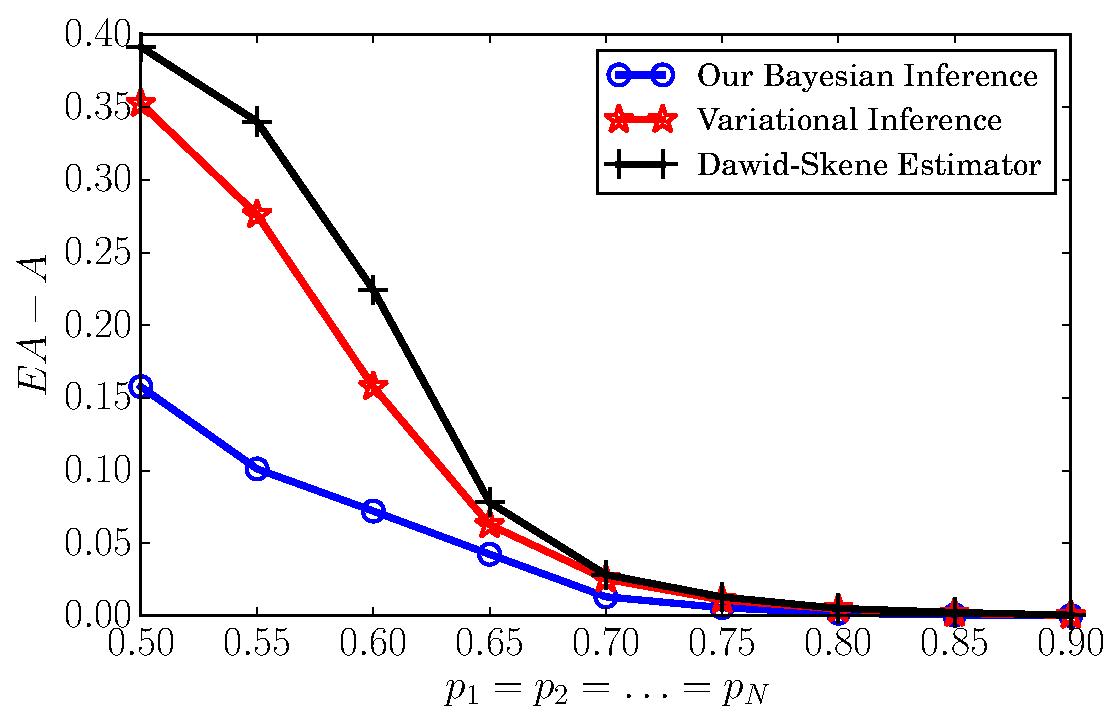
\includegraphics[width=\textwidth]{image/EXPC1}
        \caption{\label{BIM1}}
    \end{subfigure}
    ~
    \begin{subfigure}[t]{0.24\textwidth}
        \centering
        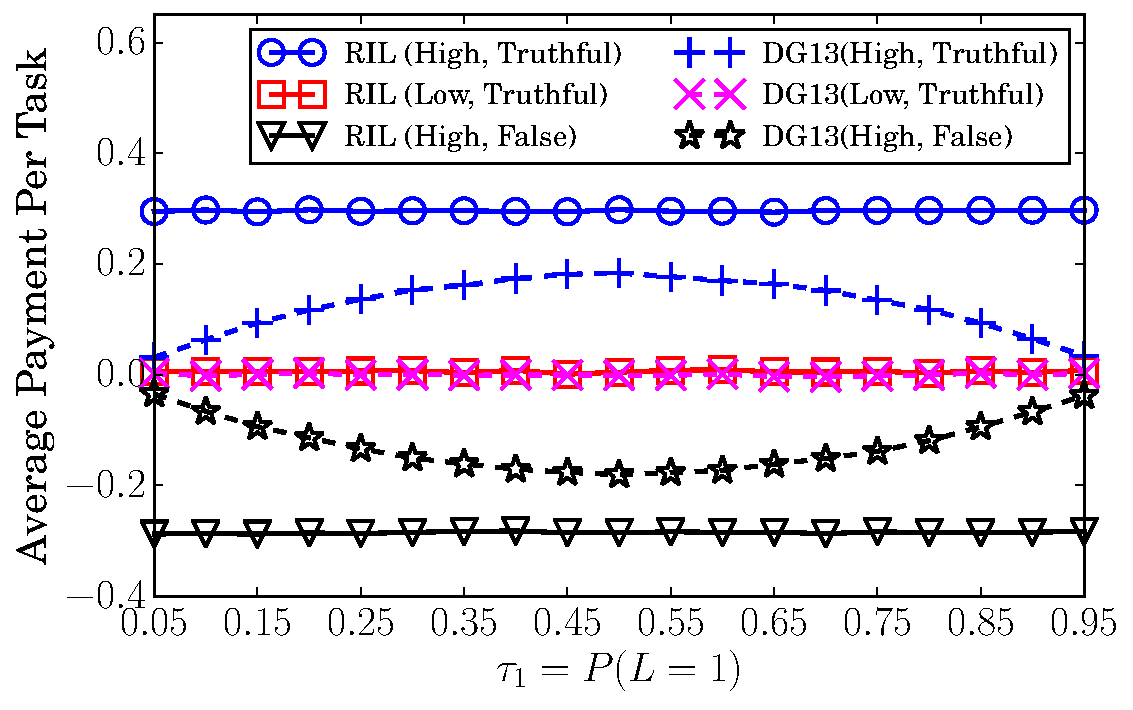
\includegraphics[width=\textwidth]{image/BPP1}
        \caption{\label{BIM2}}
    \end{subfigure}%
    ~
    \begin{subfigure}[t]{0.24\textwidth}
        \centering
        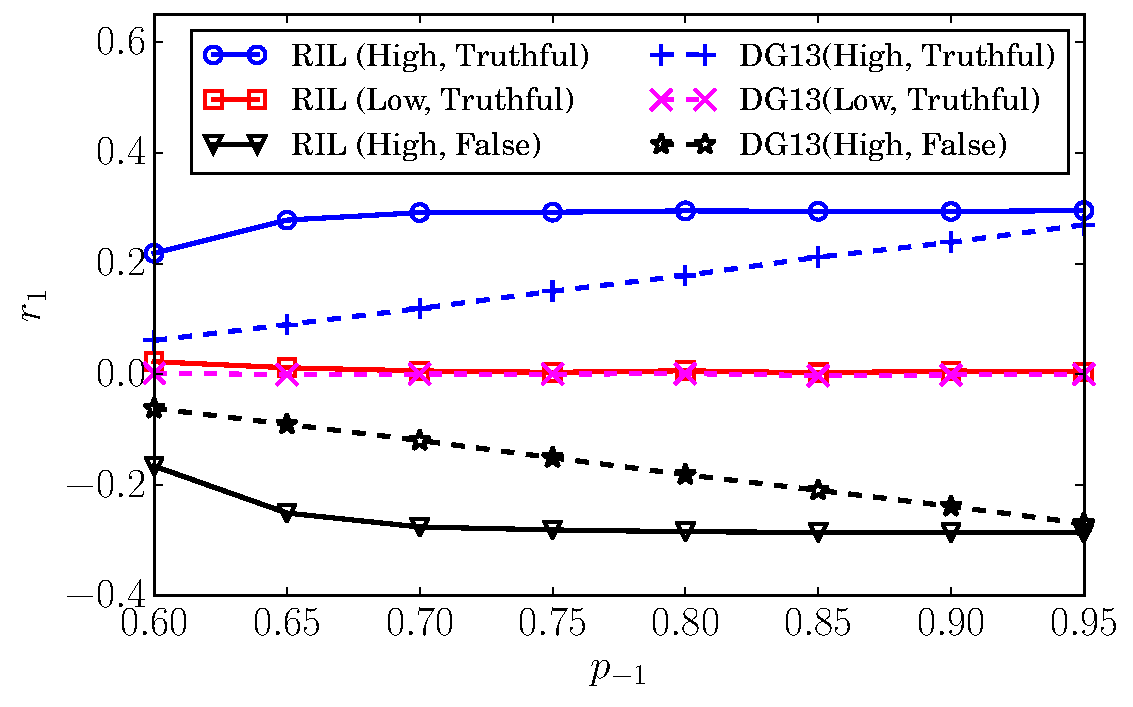
\includegraphics[width=\textwidth]{image/BPP2}
        \caption{\label{BIM3}}
    \end{subfigure}
        ~
    \begin{subfigure}[t]{0.24\textwidth}
        \centering
        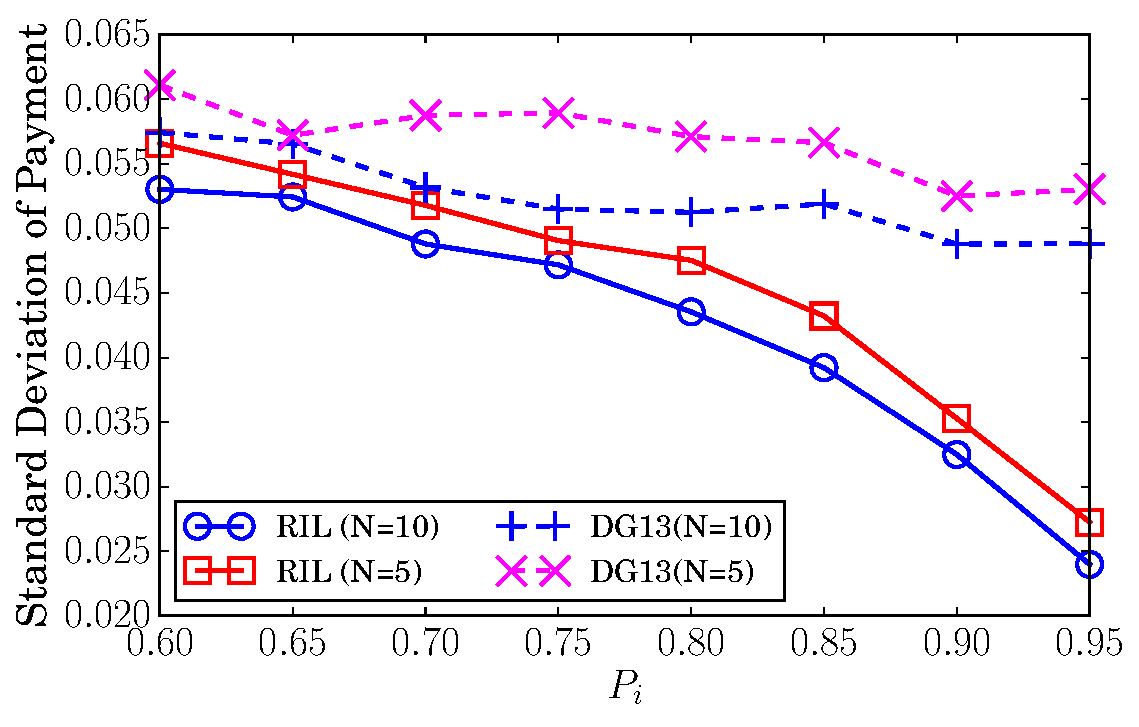
\includegraphics[width=\textwidth]{image/BPP3}
        \caption{\label{BIM4}}
    \end{subfigure}
    \vspace*{-3mm}
    \caption{\label{BIM}Empirical analysis on our one-step Bayesian incentive mechanism (BIM) (a) the inference bias (b) the reward variation as the distribution of true labels (c) the reward variation as the score of other workers (d) the standard variance of the reward for worker $1$}
\end{figure*}

\section{Empirical Experiments}
In this section, we conduct experiments on our Bayesian incentive mechanism at first to verify its advantages to lower the inference bias and improve the fairness and stability of the rewards for workers.
Then, to verify the advantage of our reinforcement incentive mechanism to boost the utility of the data requester, we empirically test our mechanism by using three representative worker models, including fully rational, bounded rational and self-learning agents.

\subsection{Bayesian incentive mechanism experiments}
In the literature of crowdsourcing, the Dawid-Skene estimator is the most popular method used to infer the true labels~\cite{dawid1979maximum,raykar2010learning}.
The variational inference estimator, which has the similar Bayesian model to our inference algorithm, is also widely-adopted in the existing studies of crowdsourcing~\cite{liu2012variational,chen2015statistical}.
To compare different estimators, we set $M=100$ and $N=10$ in Figure~\ref{BIM1}. Also, we let the score of all workers be equal, namely $p_1= \ldots=p_N$, and increase the value of $p_i$ from $0.5$ to $0.9$. Meanwhile, we set the true label distribution as the uniform distribution, namely $\tau_1=\tau_2=0.5$. For a given $p_i$, we firstly generate the true labels and then the labels of all workers both by the Bernoulli distribution. For each value of $p_i$, we run the experiments for $1000$ rounds. To show the bias of inference, we calculate the average value differences between the posterior expected accuracy $\mathbb{E}A$ and the real accuracy $A$. From the figure, we can find that, when workers can provide not-so-bad labels ($p_i>0.75$), both the two above estimators and our inference algorithm have very small bias, which agrees with the good performance of these estimators in the literature~\cite{raykar2010learning,liu2012variational}. However, if workers can only provide low-quality labels, the bias of the Dawid-Skene and variational inference estimators will become unacceptable, because the difference can be larger than $0.3$ while both $\mathbb{E}A$ and $A$ belong to $[0.5,1.0]$. In this case, we cannot use $\mathbb{E}A$ to calculate the utility of the data requester as Equation~\ref{utility}. By contrast, the bias of our Bayesian inference algorithm is much smaller, which is the foundation of our reinforcement incentive mechanism.


In Figures~\ref{BIM}b-d, we focus on $r_1$, namely, the per-task-reward received by worker $1$. Here, DG13~\cite{dasgupta2013crowdsourced,liu2017sequential}, which is the state-of-the-art incentive mechanism for binary labels, is employed as the benchmark.
DG13 decides the reward for a worker by comparing his labels with the labels provided by another randomly selected worker.
By elaborately designing the reward rules, it can also ensure reporting truthfully and exert high efforts to be a Nash equilibrium for all workers.
In all these experiments, we set $p_H=0.8$, $p_L=0.5$, and keep the other settings the same as those in Figure~\ref{BIM1}.

In Figure~\ref{BIM2}, we let $p_{-1}=p_H$, where the subscript $-1$ denotes all the workers except for worker $1$.
We change the distribution of true labels by increasing $\tau_1$ from $0.05$ to $0.95$ and compare the average values of $r_1$ corresponding to the different strategies of worker $1$.
In Figure~\ref{BIM3}, we fix the distribution of true labels to be the uniform distribution, namely, $\tau_1=\tau_2=0.5$, and increase $p_{-1}$ from $0.6$ to $0.95$.
From these two figures, we can find that the rewards provided by our mechanism are almost not affected by the variation of the distribution of true labels and the strategies of the other workers.
This observation reveals that $\mathbb{E}\tilde{p}_1$ converges to $p_1$ in most cases.
The only exception is $p_{-1}<0.7$ in Figure~\ref{BIM3} where the low-quality labels will lead to a remarkable bias of inference.
Even in this case, worker $1$ can only get the maximal reward when $p_1=p_H$, which shows the attracting ability of our mechanism to induce truthful reports and high efforts.
By contrast, $r_1$ in DG13 is severely affected by the distribution of true labels and the strategies of other workers.
For example, in Figure~\ref{BIM3}, if the other workers lower their efforts, the reward received by worker $1$ will also decrease, although worker $1$ never changes his strategies.
Thereby, for worker $1$, our Bayesian incentive mechanism is much fairer than DG13.

In Figure~\ref{BIM4}, we set $\tau_1=\tau_2=0.5$ and $p_{-1}=p_H$. We change worker $1$'s strategies by increasing $p_1$ from $0.6$ to $0.95$. Under these settings, the average values of $r_1$ corresponding to our mechanism and DG13 both can reflect the variation of $p_1$ very well. Thus, we focus on the standard variance comparison of $r_i$ in Figure~\ref{BIM4}.
If the variance is very large, the reward received by worker $1$ when $p_1=p_H$ may become lower than the reward when $p_1<p_H$.
If this case happens, it will significantly discourage worker $1$.
For example, in Figure~\ref{BIM2}, when $\tau_1=0.05$, for DG13, the difference between $r_1(p_1=p_H)$ and $r_1(p_1=0.5)$ is around $0.06$.
On the other hand, from Figure~\ref{BIM4}, the standard variance of $r_1$ is around $0.052$, which means there is a quite high probability for $r_1(p_1=p_H)<r_1(p_1=0.5)$.
From Figure~\ref{BIM4}, we can find that our Bayesian incentive mechanism has a lower variance than DG13.
If we take the fairness of our mechanism into consideration, we can conclude that our mechanism is more stable than DG13 in inducing truthful reports and high efforts from workers.


%\begin{equation}
%P(L(j)=1)=\tau_1{\prod}_{k\neq i}p_H^{\delta_{kj1}}(1-p_H)^{\delta_{kj2}}
%\end{equation}
%where $\lambda_0=\log(\tau_1/\tau_2)$ and $\lambda_i=\log(p_i/\bar{p}_i)$. For worker $i$, we assume that all other workers report truthfully and exert high efforts. Suppose the real true label is $1$. In order to ensure $\mathbb{E}[m/M]$ to approach $0$, the probability ratio in Equation~\ref{Ratio} must be positive with almost $1.0$ probability. Thus, we can directly discard the absolute operation in Equation~\ref{vot} and calculate the expected value of task $j$ as
%\begin{equation}
%\mathbb{E}_1v(j)\approx \lambda_0+(N-1)(2p_H-1)\lambda_H+(2p_i-1)\lambda_i.
%\end{equation}
%Similarly, if the real true label is $2$, then
%\begin{equation}
%\mathbb{E}_2v(j)\approx -\lambda_0+(N-1)(2p_H-1)\lambda_H+(2p_i-1)\lambda_i.
%\end{equation}
%Thus, the average task value $v$ satisfies
%\begin{equation}
%\begin{split}
%&\mathbb{E}v = \tau_1 \mathbb{E}_1v(j) + \tau_2\mathbb{E}_2v(j)\\
%&=(2\tau_1-1)\lambda_0+(N-1)(2p_H-1)\lambda_H+(2p_i-1)\lambda_i.
%\end{split}
%\end{equation}
%
%Suppose the true label is $1$.
%\begin{equation}
%x= \log\frac{P(L=1)}{P(L=2)}=g+\sum_{i=1}^{N}f(x_i,y_i,w_i,z_i)
%\end{equation}
%\noindent where $g=g_1-g_2$, and 
%\begin{equation*}
%g_1=\log(s_1+t_2+1)\;,\;g_2=\log(s_2+t_1+1).
%\end{equation*}
%Omitting the subscript in $f$, we can have $f=f_1-f_2$ with probability $p$ and $f=f_2-f_1$ with probability $1-p$. Here,
%\begin{equation*}
%f_1=\log(x+z+2)\;,\;f_2=\log(w+y+1).
%\end{equation*}
%Thus, we can have
%\begin{equation}
%\mathbb{E}g = \mathbb{E}g_1-\mathbb{E}g_2 \;,\;
%\mathbb{E}f = (2p-1)(\mathbb{E}f_1-\mathbb{E}f_2).
%\end{equation}
%From the previous proof, we know that $P(m)$ is very small when $m>>1$. Thus, we mainly focus on the region where $m$ is relatively small. For a given small $m$,
%\begin{equation}
%\mathbb{E}_{s_1, t_2}g_1\approx \mathbb{E}_{t_2}\log(np+t_2+1)
%\end{equation}
%\begin{equation}
%\log(np+t_2+1) = \log(np+1)+\sum_{i=1}^{\infty}(-1)^{i-1}q^i
%\end{equation}
%\begin{equation}
%q = \frac{t_2}{np+1}\Rightarrow 0\leq q^{i} \leq c^{i}\cdot \left(\frac{m}{M}\right)^i\leq c^{i}\frac{m}{M}
%\end{equation}
%Then,
%\begin{equation}
%\mathbb{E}g_1 \approx \mathbb{E}_{m}\log(1+Mp-mp)
%\end{equation}
%\begin{equation}
%\log(1+Mp-mp)\approx\log(1+Mp)+\sum_{i=1}^{\infty}(-1)^{i}\left(\frac{m}{M}\right)^i
%\end{equation}
%Using the similar way of approximation for the computation of $\mathbb{E}g_2$, $\mathbb{E}f_1$ and $\mathbb{E}f_2$, we can have
%\begin{equation}
%\begin{split}
%\mathbb{E}g_1\approx \log(Mp)\;,\;\mathbb{E}g_2\approx \log(M(1-p))\\
%\mathbb{E}f_1\approx \log(Mp)\;,\;\mathbb{E}f_2\approx \log(M(1-p))
%\end{split}
%\end{equation}
%Thus, if all workers exert high efforts and report truthfully,
%\begin{equation}
%    \mathbb{E}x \approx \log\lambda_0 + {\sum}_{i=1}^{N}\log\lambda_{i,H}
%\end{equation}
%If the true label is $2$, then
%\begin{equation}
%    \mathbb{E}x \approx \log\lambda_0 - {\sum}_{i=1}^{N}\log\lambda_{i,H}
%\end{equation}
%Thereby,
%\begin{equation}
%    \mathbb{E}|x|\approx (2p_0-1)\log\lambda_0+ {\sum}_{i=1}^{N}\log\lambda_{i,H}
%\end{equation}
%When, for example, worker $1$ deviate from the desired equilibrium strategy, the non-equilibrium state correspond to
%\begin{equation}
%    \mathbb{E}|x'|\approx (2p_0-1)\log\lambda_0+ \log\lambda_{1}+{\sum}_{i=2}^{N}\log\lambda_{i,H}
%\end{equation}
%The minimal value of $\mathbb{E}|x'|$ is reached when worker $1$ exert high efforts and report falsely, namely $\log\lambda_{i}=-\log\lambda_{i,H}$.
%Thus, the maximal reward increment brought by worker $1$'s strategy switch is
%\begin{equation}
%    V_1 = F(\mathbb{E}x)-F(\mathbb{E}x') \approx 2\log\lambda_{1,H}\cdot \left.\frac{\mathrm{d}F}{\mathrm{d}x}\right|_{x=x_H}
%\end{equation}
%Since $p_0$ is difficult to estimate, we define the upper bound of the value increment as
%\begin{equation}
%    V = 2\max_{i}\log\lambda_{i,H} \cdot  \max_{x\in [x_H, \infty)}\frac{\mathrm{d}F}{\mathrm{d}x} 
%\end{equation}
%where $x_H= \log\lambda_0 + {\sum}_{i=1}^{N}\log\lambda_{i,H}$.
%Considering the discounted reward calculation in reinforcement learning, we can know the maximum value difference can be created by the manipulation of any worker is $(1-\rho)^{-1}V$. Meanwhile, if the reinforcement part increases the scaling factor by $\delta$ to obtain the reward increment, we need to pay more than $\sum_{i=1}^{N}M\delta (p_{i,H}-0.5)$. Thus, if we want to prevent the reinforcement learning module from the adversarial manipulation, the minimal gap $\delta$ between to two available scaling factors should satisfy
%\begin{equation}
%    \sum_{i=1}^{N}M\delta (p_{i,H}-0.5) > V.
%\end{equation}

\bibliographystyle{named}
\bibliography{ref}

\end{document}


% This document was modified from the file originally made available by
% Pat Langley and Andrea Danyluk for ICML-2K. This version was created
% by Iain Murray in 2018. It was modified from a version from Dan Roy in
% 2017, which was based on a version from Lise Getoor and Tobias
% Scheffer, which was slightly modified from the 2010 version by
% Thorsten Joachims & Johannes Fuernkranz, slightly modified from the
% 2009 version by Kiri Wagstaff and Sam Roweis's 2008 version, which is
% slightly modified from Prasad Tadepalli's 2007 version which is a
% lightly changed version of the previous year's version by Andrew
% Moore, which was in turn edited from those of Kristian Kersting and
% Codrina Lauth. Alex Smola contributed to the algorithmic style files.
